\chapter{Amplificadores Clase B y AB}


\hspace{10pt} \textbf{Ejercicio 1}: Para la  configuración de salida mostrada en
la figura \ref{eje1}, calcular la máxima potencia de salida sin
distorsión. Averiguar si el recorte a plena potencia es simétrico;
en el caso que no lo sea, calcular los picos de tensión de salida
positivo y negativo máximos, $v_O^+$ y $v_O^-$ respectivamente. ¿Qué
cambiaría del circuito para obtener más potencia de salida?. Suponer
que $V_{B3}$ es la necesaria para que $V_{occ}=0$.


\begin{figure}[h]
	\centering
	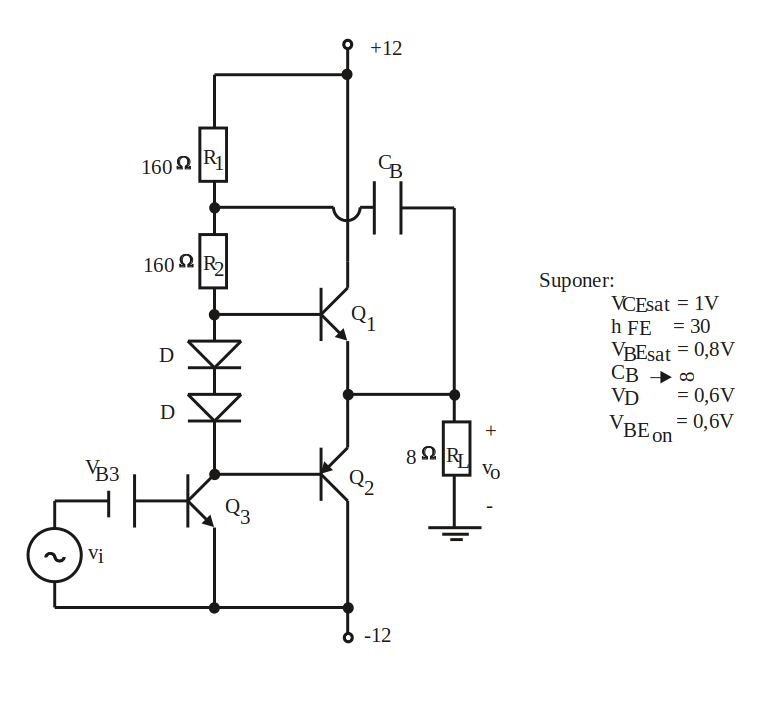
\includegraphics[width=0.8\linewidth]{figuras/claseb1.png}\\
	\caption{Ejercicio 1.}\label{eje1}
\end{figure}

\textbf{Ejercicio 2}:  En el  circuito de la figura \ref{eje2}
calcular: a) el valor de $R_5$ para que el circuito funcione
correctamente ($V_{occ}=0$);  b) máxima potencia de salida sin
distorsión.

\begin{figure}[h]
	\centering
	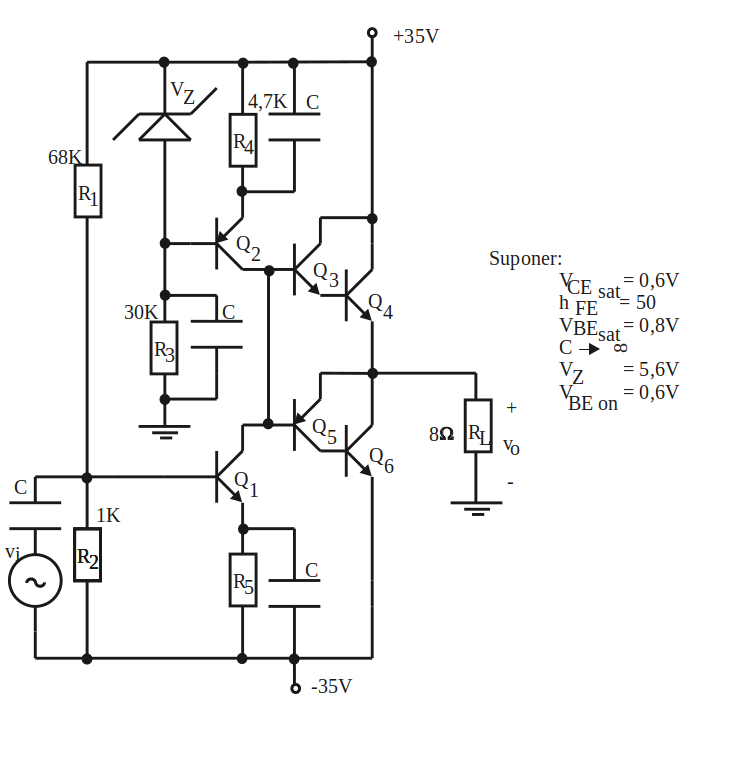
\includegraphics[width=0.8\linewidth]{figuras/claseb2.png}\\
	\caption{Ejercicio 2.}\label{eje2}
\end{figure}

\textbf{Ejercicio 3}: En una salida clase B ideal hallar
$\eta_{max}$ y $P_{Dmax}$  para cada transistor de salida,
trabajando con fuente simple para: a) onda senoidal; b)  onda
triangular y c) onda cuadrada.

\textbf{Ejercicio 4}: En el circuito de la figura \ref{eje4} se
desea que la potencia de salida sin distorsión sea $P_o = 8 W$: a)
calcular la ganancia de corriente $h_{FE}$ que deben tener los
transistores de salida si el amplificador $a$ puede entregar como
máximo una corriente de salida de 10 mA;  b)  hallar la tensión pico
de entrada para obtener los 8 W sobre $R_L$ a una frecuencia de 5
KHz y a una frecuencia de 100 KHz y c) calcular el ancho de banda
total.

\begin{figure}[h]
	\centering
	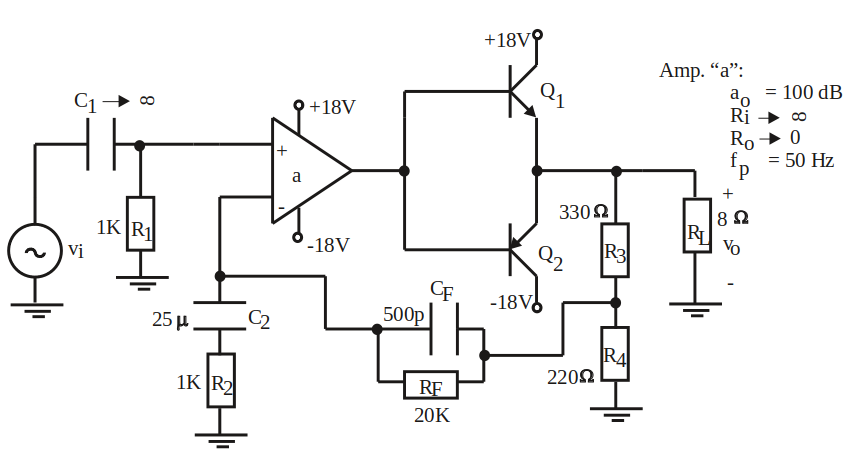
\includegraphics[width=0.8\linewidth]{figuras/claseb4.png}\\
	\caption{Ejercicio 4.}\label{eje4}
\end{figure}

\textbf{Ejercicio 5}: Dado el  circuito de la figura \ref{eje5},
calcular: a) impedancia de entrada; b) impedancia de salida;  c)
ganancia de tensión total a frecuencias medias; d) transferencia de
la red de realimentación en función de la frecuencia (graficarla) y
e) potencia disipada máxima en cada transistor de salida, disipador
necesario y rendimiento para esa condición.

\begin{figure}[h]
	\centering
	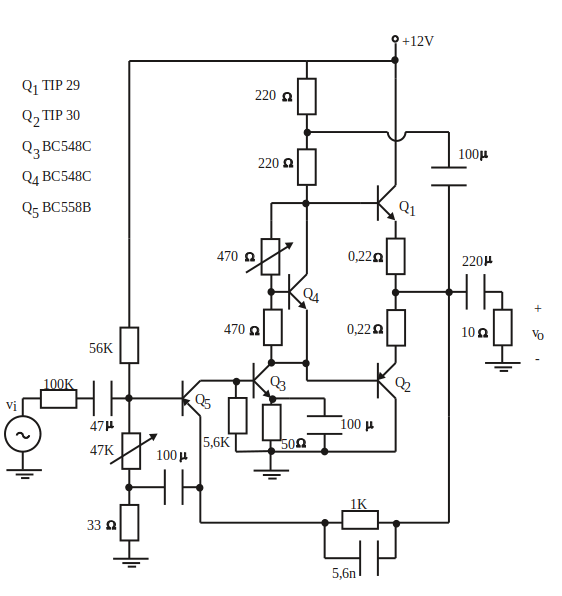
\includegraphics[width=0.8\linewidth]{figuras/claseb5.png}\\
	\caption{Ejercicio 5.}\label{eje5}
\end{figure}

\textbf{Ejercicio 6}:   Se desea obtener $P_{Lmax}=4,05 W$ sobre la
carga $R_L=10\Omega$, utilizando un circuito como el mostrado en la
figura \ref{eje6}, en el que algunos de sus componentes ya están
fijos (suponer que $C_2$ se comporta como un corto circuito para la
menor frecuencia de trabajo). a) Elegir $Q_1$ y $Q_2$ de la tabla
mostrada en dicha figura y calcular la resistencia térmica del
disipador necesario si la $T_{amb max}= 50°C$. b) Diseñar $R_2$,
$R_3$, $R_4$ y $V_1$ para lograr el objetivo (asegurar que $R_2 \geq
50\Omega$ para estabilizar la polarización de $Q_4$). c) ¿Qué ocurre
con $P_{Lmax}$ si se desconecta $C_2$?, calcular la nueva $P_{Lmax}$
si es que esta cambia.

\begin{figure}[h]
	\centering
	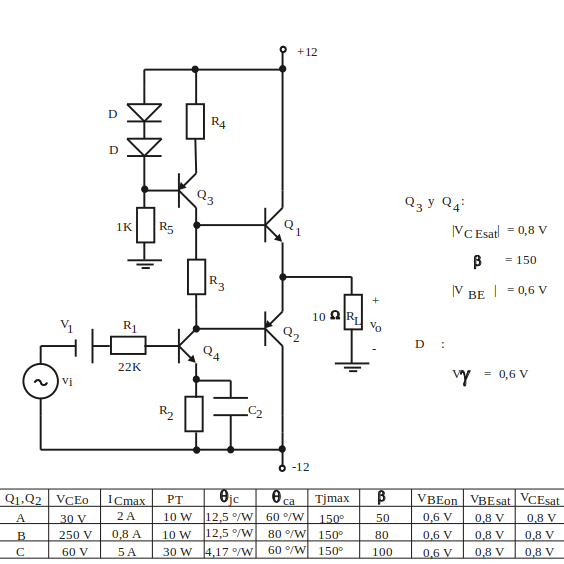
\includegraphics[width=0.8\linewidth]{figuras/claseb6.png}\\
	\caption{Ejercicio 6.}\label{eje6}
\end{figure}

\textbf{Ejercicio 7}: Diseñar la etapa de salida clase AB de la
figura \ref{eje7}, para obtener una potencia de salida máxima sin
distorsión $P_{Lmax}=20 W$ sobre una carga $R_L=8\Omega$, suponiendo
una $T_{amb max}=45°C$.

\begin{figure}[h]
	\centering
	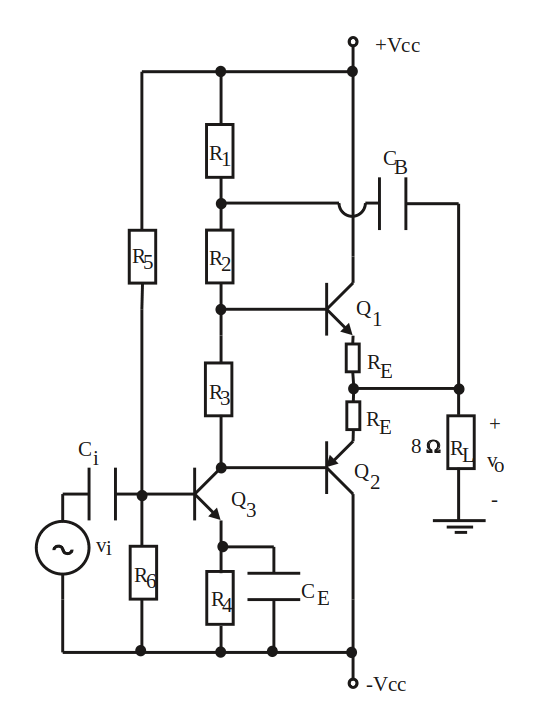
\includegraphics[width=0.6\linewidth]{figuras/claseb7.png}\\
	\caption{Ejercicio 7.}\label{eje7}
\end{figure}

